\subsection{Results}
Figure \ref{fig-timePerTask} shows the time until the correct answer was given per task. Here we consider both the results from the controlled experiment as the online experiment, to remedy the small set of subjects available for the controlled experiment. We immediately see some interesting result for task 3. We make no assumptions about the underlying distribution so we perform a non-parametric Wilcoxon Mann-Whitney U test (\textit{$H_0$: times for the Console group and RxFiddle group are drawn from the same population}) to see if the differences are significant, and a Cliffs delta test for ordinal data to determine the effect size.

\begin{centering}
% \begin{table}[]
% \centering
% \caption{My caption}
%\label{my-label}
\begin{tabular}{llllll}
\hline
            & \textbf{$n_1$} & \textbf{$n_2$} & \textbf{W} & \textbf{p-value} & \textbf{Cliffs $\delta$} \\ \hline
\textbf{T1} & 26                      & 30                       & 343        & 0.448           & 0.121     \\
\textbf{T2} & 29                      & 27                       & 362        & 0.637           & 0.0754    \\
\textbf{T3} & 22                      & 24                       & 100        & 0.000186        & 0.621     \\
\textbf{T4} & 15                      & 12                       & 86         & 0.867           & 0.0444    \\ \hline
\end{tabular}
% \end{table}
\end{centering}

For tasks T3 we can reject $H_0$ with high significance ($p < 0.05$), the RxFiddle group is faster.
For the tasks T1, T2 and T4 we can not reject $H_0$ ($p > 0.05$), and for T2 the U test indicates no difference at all, meaning the RxFiddle group and Console group perform or could perform equally.

\begin{figure}[h]
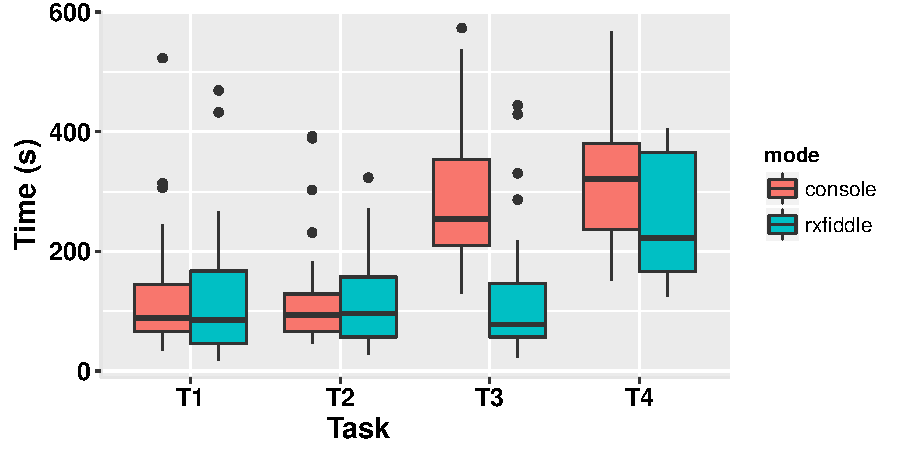
\includegraphics[width=\columnwidth]{images/timePerTask.pdf}
\caption{Time until correct answer per task}
\label{fig-timePerTask}
\end{figure}

While this could be observed as a negative result, RxFiddle is a new tool, and the users have only just been exposed to the tool and received only a short training. More importantly we regarded developers of possibly different experience levels, and developers with more Rx experience might be more familiar with the concepts that RxFiddle visualizes. To investigate this further, we split the results for different groups of subjects, as shown in Figure \ref{fig-timePerTaskSplit}.  When split (at the median value, inclusive) for years of RP experience and the self-assessed RP experience (Likert-scale) we see bigger differences for all tasks for groups with more experience. This indicates that the visualization might be less suitable for inexperienced subjects.

Even while regarding more experienced subjects, the effect is still most significant for T3. We think that RxFiddle might be more suitable to replace traditional debugging for some tasks than others.